\chapterimage{band1.png}
\chapter{Condições}\label{cap:seleccao}

Na nossa vida diária, a maior parte das acções que efectuamos estão sujeitas a determinadas condições para poderem ser realizadas. Vamos à aula de Programação Multimédia,  \textbf{se} quisermos ser os melhores a programar;) vamos à praia se não estiver a chuver; se tivermos fome, comemos; se gostarmos da comida, vamos à cantina, senão...vamos a outro lado; etc.

Também em programação necessitamos de executar acções condicionalmente, i.e., se determinadas circunstâncias se verificarem. 
Ao processo de execução condicional de determinadas secções de código do programa chamamos \emph{controlo de fluxo}.

Podemos controlar o fluxo do programa, i.e., que secções de código executam, recorrendo a estruturas de controlo
de fluxo. Essas estruturas são duas: \texttt{if} e \texttt{switch}.


\section{Se Isto Então Aquilo (\texttt{if})}
\begin{figure}[!ht]
	\centering
		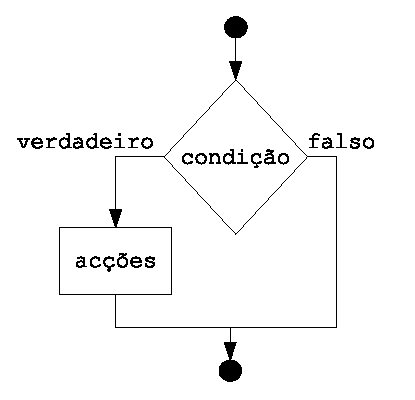
\includegraphics[width=5cm]{images/se-entao.eps}
	\caption{\texttt{if else} -- Diagrama de Fluxo}
	\label{fig:se-entao}
\end{figure}
A estrutura \texttt{if}, permite-nos executar condicionalmente um conjunto de instruções.
Na sua forma mais básica, a estrutura reduz-se a:
\begin{lstlisting}
if (<condição>) {
    [acções]
}
\end{lstlisting}

Por exemplo:
\begin{lstlisting}
int x;

x = 5;

if (x > 10) {
    print("X é maior do que 10.");
}
\end{lstlisting}
Neste caso, a frase ``X é maior do que 10'' apenas é escrita se
o valor de \texttt{x} for superior a 10. Caso contrário a instrução
de escrita é simplesmente ignorada. A Figura~\ref{fig:se-entao} mostra o diagrama de fluxo da estrutura
\texttt{if}. Esta estrutura é composta por duas partes fundamentais:
\begin{description}
\item[condição] 
A condição é a situação que queremos testar. No caso do exemplo, queriamos saber se a variável \texttt{x} tinha um valor superior a 10.

\item[acções]
São as instruções que queremos executar se a condição for \textbf{verdadeira}. As instruções a executar são delimitadas por duas chavetas (``\{'' e ``\}''). As chavetas, em Processing, servem para delimitar um \emph{bloco de código}. No caso do \texttt{if}, o bloco de código é um conjunto de instruções (podemos ter várias instruções) executado se a condição for verdadeira.
\end{description}

E se quisermos testar também a condição inversa? Ou seja, falsa?

Uma das opções seria (no caso do exemplo anterior)%
\footnote{A condição inversa de ``x maior do que 10'' é ``x menor ou igual a 10''.}%
:
\begin{lstlisting}
int x;

x = 5;

if (x > 10) {
    print("X é maior do que 10.");
}
if (x <= 10) {
    print("X é menor ou igual a 10.");
}
\end{lstlisting}
Neste exemplo conseguimos determinar se ``x maior do que 10'' e também se ``x menor ou igual a 10''. No entanto, o Processing, fornece-nos uma forma mais rápida (em termos de escrita de código) de conseguir isto:
\begin{lstlisting}
int x;

x = 5;

if (x > 10) {
    print("X é maior do que 10.");
} else {
    print("X é menor ou igual a 10.");
}
\end{lstlisting}

A \emph{keyword} \texttt{else} serve para executar um conjunto de instruções caso a condição do \texttt{if} seja falsa. De novo, o conjunto de instruções a executar é delimitado por chavetas.
O diagrama desta estrutura (\texttt{if else}) é apresentado na Figura~\ref{fig:se-entao-senao}.

\begin{figure}[!ht]
	\centering
		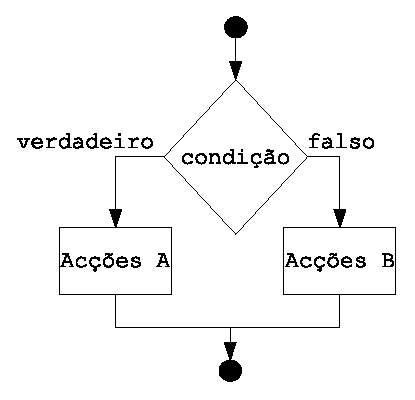
\includegraphics[width=5cm]{images/se-entao-senao.eps}
	\caption{\texttt{if else} -- Diagrama de Fluxo}
	\label{fig:se-entao-senao}
\end{figure}

A estrutura \texttt{if} pode ser utilizada em ``cascata'', i.e., podemos testar várias condições consecutivamente:
\begin{lstlisting}
int x;

x = 5;

if (x > 10) {
    print("X é maior do que 10.");
} else if (x > 5) {
    print("X é maior do que 5.");
} else if (x > 1) {
    print("X é maior do que 5.");
} else {
    print("X é menor ou igual a 1.");
}
\end{lstlisting}


\begin{figure}[ht]
	\centering
		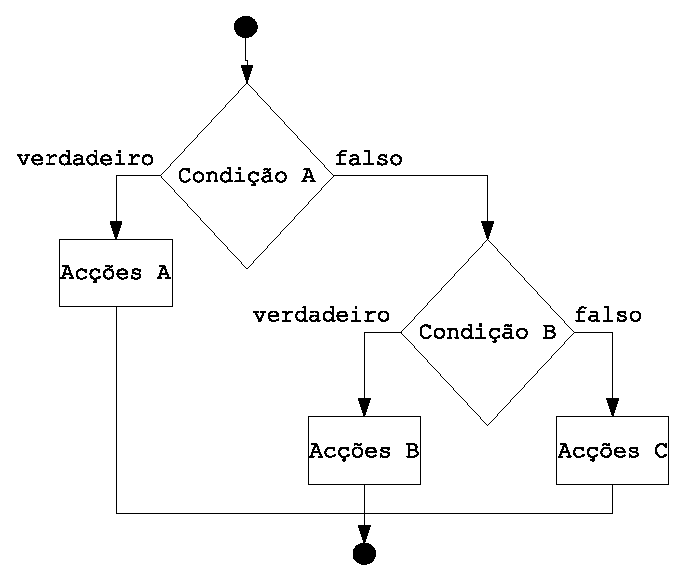
\includegraphics[width=8cm]{images/se-entao-senao-se-senao.eps}
	\caption{\texttt{if else if} -- Diagrama de fluxo}
	\label{fig:se-entao-senao-se-senao}
\end{figure}

Nesta variante, as condições são testadas sequencialmente. Se alguma das condições for
satisfeita, as acções associadas serão executadas e o programa sairá da estrutura, ou seja,
apenas um dos conjuntos de instruções pode ser executado. A Figura~\ref{fig:se-entao-senao-se-senao}
mostra o diagrama de fluxo correspondente.

Obviamente, que o conjunto de instruções executado caso a condição seja verdadeira (ou falsa) pode conter ele mesmo outras estruturas \texttt{if} (o \texttt{if} é uma instrução como outra qualquer):
\begin{lstlisting}
int x;
int y;

x = 5;
y = 7;

if (x > 10) {
    print("X é maior do que 10.");
    if (y > 5) {
        print("Y é maior do que 5.");
    }
} 
\end{lstlisting}
Neste exemplo, escrevemos a mensagem \emph{``X é maior do que 10.''} se \texttt{x} for maior do que 10 e escrevemos a mensagem 
\emph{``Y é maior do que 5.''} se \texttt{x} for maior do que 10 e ao mesmo tempo \texttt{y} for maior do que 5.

\section{Comutar (\texttt{switch})}

\begin{figure}[!h]
	\centering
		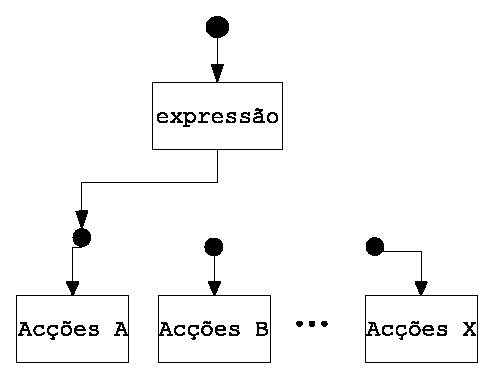
\includegraphics[width=6cm]{images/comuta.eps}
	\caption{\texttt{switch} -- Diagrama de fluxo}
	\label{fig:comuta}
\end{figure}

A estrutura \texttt{switch} é uma forma mais prática, nalguns casos, de escolher um
caminho de entre vários possíveis. É utilizado um valor inteiro para decidir
qual o caminho a executar:
\begin{lstlisting}
int x;

switch (x) {
    case 1: 
        /* instruções a executar se x for igual a 1	*/
        break;
	
    case 2: 
        /* instruções a executar se x for igual a 2	*/
        break;
	
    case 4: 
        /* instruções a executar se nenhum dos anteriores for executado	(opcional) */
        break;	    
}
\end{lstlisting}

O \texttt{switch} é composto por duas secções:
\begin{description}
\item[expressão de teste] 
A expressão de teste é normalmente uma variável do tipo \texttt{int}. Por exemplo, se tivermos uma variável que representa uma opção do utilizador, que pode ir de 1 a 5, podemos ter acções diferentes para cada opção.
	
\item[acções para para caso]
São as instruções a executar se a variável tiver o valor do caso actual. As instruções devem sempre terminar com a instrução \texttt{break}%
\footnote{A keyword \texttt{break} é utilizada para ``partir'' o fio de execução do programa nalgumas situações. No caso do \texttt{switch}, o \texttt{break} faz com que o programa saia da estrutura \texttt{switch}.}%
.
\end{description}



\section{Opero...Se... (Operadores Condicionais)}

Até agora vimos apenas um tipo de condição ``x \textbf{maior do que}...''. No entanto, existem mais condições que podemos testar:
\begin{itemize}
\item Igual a ($==$)%
\footnote{O operador condicional de ``igual a'' é o símbolo $==$ para se distinguir do operador de atribuição $=$ de variáveis.}%
;
\item Maior do que ($>$);
\item Menor do que ($<$);
\item Maior ou igual a ($>=$);
\item Menor ou igual a($<=$);
\item Diferente de ($!=$)
\end{itemize}

Os símbolos entre parentesis são os chamados \emph{operadores condicionais}.
Os operadores condicionais podem ser usados sobre dados de vários tipos (inteiros, reais, lógicos). O resultado da operação é um valor lógico: verdadeiro ou falso.

Os operadores condicionais são utilizados sobretudo no controlo de fluxo do programa e nas condições 
de paragem dos ciclos (explicado no capítulo seguinte). No entanto podemos atribuir o resultado de uma operação
condicional a uma variável lógica:
\begin{lstlisting}
boolean maior;

maior = 1 > 3;
\end{lstlisting}
Neste caso, o valor de \texttt{maior} seria \texttt{false}%
\footnote{A \emph{keyword} \texttt{false} é um valor especial do Processing que pode ser atribuido a variáveis lógicas. De igual modo, existe a \emph{keyword} \texttt{true}.}%
.

\subsection{Lógicos} 
Nos exemplos com condições que vimos até agora, todas as condições eram simples: ``x maior do que 10'', ``y maior do que 5'', etc. No entanto, as condições a testar podem ser bastante mais complexas.

Na vida real, pensamos muitas vezes coisas do género: ``se o FCP ganhar o jogo \textbf{e} o SLB perder, o FCP ganha o campeonato'', ou ``se o SCP ganhar \textbf{ou} o SLB empatar, o FCP perde o campeonato'' ou ``se eu \textbf{não} passar no exame de condução, vou ter de o repetir''.
Todas estas situações representam condições complexas que não são mais do que a conjugação de várias condições simples: ``o FCP ganhar o jogo'', ``o SLB perder o jogo'', ''passar no exame de condução'', etc. Estas condições simples, são ligadas através do que se designa, em programação, por \emph{operadores lógicos}: \textbf{e}, \textbf{ou} e \textbf{não}. 

Os operadores condicionais servem ligar condições simples, de modo a criar condições mais complexas. O valor da condição complexa resultante (verdadeira ou falsa) depende do valor de cada condição simples.

Os símbolos utilizados em Processing para representar estes operadores são os seguintes:
\begin{center}
\begin{tabular}{lll}
Operador & Símbolo & Descrição\\
\hline
	\textbf{e} &\texttt{\&\&} &dois ``\&'' (e comercial).\\
	\textbf{ou} &\texttt{||} &dois ``|'' (\emph{pipeline} -- símbolo que se encontra\\
	& & por cima da barra invertida ``$\backslash$'' no teclado).\\
	\textbf{não} &\texttt{!} &um ``!'' (ponto de exclamação).\\
\end{tabular}
\end{center}

Os operadores lógicos (``ou'', ``e'', ``não'') operam sobre dados lógicos. Os operadores ``ou'' e
``e'' são operadores binários (operam sobre dois operandos); o operador ``não'' é um operador unário. As tabelas 
de verdade%
\footnote{Uma \emph{tabela de verdade} é uma tabela que indica o resultado da conjugação de um operador lógico com todos os valores possíveis dos operandos.}
 de cada operador são as seguintes:
\begin{center}
\begin{tabular}{c|c|c}
\multicolumn{3}{c}{\texttt{||} -- (``ou'')}\\
\hline
A & B & A \texttt{||} B\\
\hline
\texttt{false} & \texttt{false} & \texttt{false}\\
\texttt{false} & \texttt{true} & \texttt{true}\\
\texttt{true} & \texttt{false} & \texttt{true}\\
\texttt{true} & \texttt{true} & \texttt{true}\\
\end{tabular}
\end{center}

\begin{center}
\begin{tabular}{c|c|c}
\multicolumn{3}{c}{\texttt{\&\&} -- (``e'')}\\
\hline
A & B & A \texttt{\&\&} B\\
\hline
\texttt{false} & \texttt{false} & \texttt{false}\\
\texttt{false} & \texttt{true} & \texttt{false}\\
\texttt{true} & \texttt{false} & \texttt{false}\\
\texttt{true} & \texttt{true} & \texttt{true}\\
\end{tabular}
\end{center}

\begin{center}
\begin{tabular}{c|c}
\multicolumn{2}{c}{\texttt{!} -- (``não'')}\\
\hline
A & \texttt{!}A\\
\hline
\texttt{false} & \texttt{true}\\
\texttt{true} & \texttt{false} \\
\end{tabular}
\end{center}

Uma vez que o resultado de uma operação condicional é um valor lógico, podemos combinar operações condicionais
e lógicas:
\begin{lstlisting}
boolean maisAltoEMaisVelho = (idadeJoao > idadeAna) e (alturaJoao > alturaAna);
\end{lstlisting}
Neste caso \texttt{maisAltoEMaisVelho} será \texttt{true} apenas se a idade do João
for superior à idade da Ana e se ele for também mais alto. A utilização dos parêntesis, neste
caso, não era absolutamente necessária porque os operadores condicionais têm precedência
sobre os operadores lógicos. No entanto, a sua utilização facilita a leitura do código.

\section{Um Exemplo Prático}
Tendo conhecimentos destes novos operadores -- condicionais e lógicos -- podemos escrever programas mais complexos.

O exemplo seguinte é um programa que consiste num quadrado branco que sobe e desce no ecrã. A única informação (variáveis) que precisamos de manter é a posição vertical actual do quadrado e a velocidade a que se desloca (quantos pixeis se mexe de cada vez). 
\begin{center}
	
\includegraphics[width=4cm]{images/condicaoRectanguloCimaBaixo.eps}
\end{center}
\begin{lstlisting}[caption=Testar a posição vertical de um rectângulo, label=exe:condicaoRectanguloCimaBaixo]
int y;          //a posição do quadrado
int velocidade; //a velocidade (pode ser negativa)

void setup() {
    size (200, 200);
    
    y = 0;
    velocidade = 5;
}


void draw() {
    background(0);       //limpar o ecra
    
    rect(100, y, 10, 10); //desenhar o rectangulo na posicao vertical y
    
    y = y + velocidade;   //actualizar a posicao
        
    if (y > 200) {        // se o rectangulo passou o fundo do ecra, inverter a velocidade
        velocidade = -5;
    }
    if (y < 0) {          // se o rectangulo passou o cimo do ecra, inverte a velocidade
        velocidade = 5;
    }
}
\end{lstlisting}
O rectângulo é desenhado com a instrução \texttt{rect(100, y, 10, 10)}%
\footnote{A instrução \texttt{rect()} precisa de quatro parâmetros: a posição x e y e a largura e altura do rectângulo.}
de forma que o rectângulo é desenhado na posição vertical dada pela variável \texttt{y}.
Uma vez que a variável \texttt{y} é actualizada com o valor da velocidade, isto faz com que o rectângulo seja desenhado sempre numa posição diferente, dando a ilusão de movimento contínuo.

Para verificarmos se o rectângulo bateu numa das paredes (limites da janela, inferior ou superior) basta-nos testar a posição vertical. Uma vez que sabemos qual a dimensão da janela (200x200), sabemos que se a posição \texttt{y} for superior a 200, então o rectângulo bateu na parede inferior (lembrem-se que o y ``cresce'' para baixo). De igual modo se a posição for inferior a 0, bateu na parede superior.



\section{Exercícios}
\begin{enumerate}
	
	\item \label{exe_4_operadores} 
	* Determine o resultado lógico das seguintes expressões, sabendo que ($a = 13, b = 2, c = 3, n = verdadeiro, p = falso$):
\begin{enumerate}
\item $a == b$ 
\item $a < b$
\item $a > b > c$
\item $!(a > b)$
\item $! !(a > b)$
\item $(a > b) \&\& (b > c)$
\item $!((a > b) \&\& (b > c))$
\item $(!(a > b)) \&\& (b > c)$
\item $n || p$
\item $(a>b) \&\& p$
\item $!((a>b) \&\& p)$\item Nas expressões anteriores, em que o resultado é \emph{falso}, determine valores para $a$, $b$ e $c$ de
modo a torná-las \emph{verdadeiro}.
\end{enumerate}

\item \label{exe_4_fluxo}
* Escreva os programas para resolver os seguintes problemas:
\begin{enumerate}

\item Determinar a média de dois valores inteiros. Escrever o valor da média
se esta for superior a 100. Assuma que os valores estão armazenados nas variáveis $a$ e $b$.

\item Determinar se um valor é positivo, negativo ou zero. Assuma que o valor está armazenado na variável $a$.

\item Determinar se um valor (gerado aleatoriamente) é par ou ímpar. 

\item Determinar, de entre dois valores, o maior e o menor (ou se são iguais). Por exemplo, se os dois valores forem 4 e 2, o 
programa deve escrever: 
\begin{lstlisting}
"O maior valor é 4"
"O menor valor é 2"
\end{lstlisting}
Se os valores forem 2 e 2, deve escrever:
\begin{lstlisting}
"Os valores são iguais"
\end{lstlisting}
Assuma que os valores estão armazenados nas variáveis $a$ e $b$.

\item Determinar se uma coordenada ($x, y$), introduzida pelo utilizador, está dentro de um rectângulo definido definido pelos seus cantos superior esquerdo ($x0, y0$) e inferior direito ($x1, y1$). O programa deve apresentar o resultado ao utilizador: ``A coordenada está dentro do rectângulo'' ou ``A coordenada está fora do rectângulo''. \label{xpto}

\item Determinar o máximo de três valores. Assuma que os valores estão armazenados nas variáveis $a$, $b$ e $c$.

\item Determinar o máximo de cinco valores.
Assuma que os valores estão armazenados nas variáveis $a$, $b$, $c$, $d$ e $e$.
\end{enumerate}

	\item \label{exe:4_1}
	* Altere o Projecto \ref{ps:linhaAnimada} do capítulo anterior, de modo a que a linha se mantenha sempre dentro do ecrã e sempre animada.
\end{enumerate}